% Canonical Chapter 18; the web edition is synchronized from this source.
\chapter[Inverse Dynamics and the Parallel Loop Problem]{Inverse Dynamics and\\the Parallel Loop Problem}
\label{ch:inverse_dynamics_parallel}

A swing can reveal how the club moved without revealing how each hand loaded it.
A measured hand wrench can reveal an arm's net joint loading without identifying
every muscle force. A forward simulation can predict a specified intervention
without establishing that a golfer actually used that strategy. These are three
different questions, and each deserves a complete answer at its own level.

The purpose of inverse dynamics is to determine loads consistent with measured
motion, declared mechanics, and known boundary conditions. Its value does not
depend on recovering every muscle's contribution. The research challenge is to
identify which combinations of loads the available measurements determine, which
remain ambiguous, and which additional measurements would distinguish competing
explanations of the golf swing.

\section{Start With the Quantity Being Investigated}
\label{sec:inverse_definition}

An analysis should name its target before choosing an algorithm. Clubhead speed,
clubface orientation, net hand wrench, shoulder moment, muscle force, mechanical
work, metabolic demand, and tissue stress are not interchangeable outputs.
They require different boundaries, models, and evidence. A joint moment is not
an electrical activation signal; a ground moment is not a direct measurement of
pelvis acceleration; and neither one alone measures energy supplied to the club.

For example, suppose two golfers deliver the same club pose and velocity at
impact. They need not have followed the same earlier trajectory. Even identical
full club trajectories need not imply identical hand loading. Identical
skeletal trajectories and boundary loads can still admit multiple muscle-force
patterns. Conversely, additional sensors or sufficiently restrictive mechanics
can make a particular load identifiable. The conclusion must follow from the
specified inverse problem rather than the slogan that closed loops are always
ambiguous.

Motion capture supplies image or marker observations. Segment poses, joint
coordinates, and their derivatives are estimates obtained through calibration,
kinematic fitting, smoothing, and differentiation. External forces require
instruments or a declared force model; they are not automatically another output
of differentiating joint angles. A complete report carries that chain of
inference into its final uncertainty estimates.


\begin{figure}[htbp]
\centering
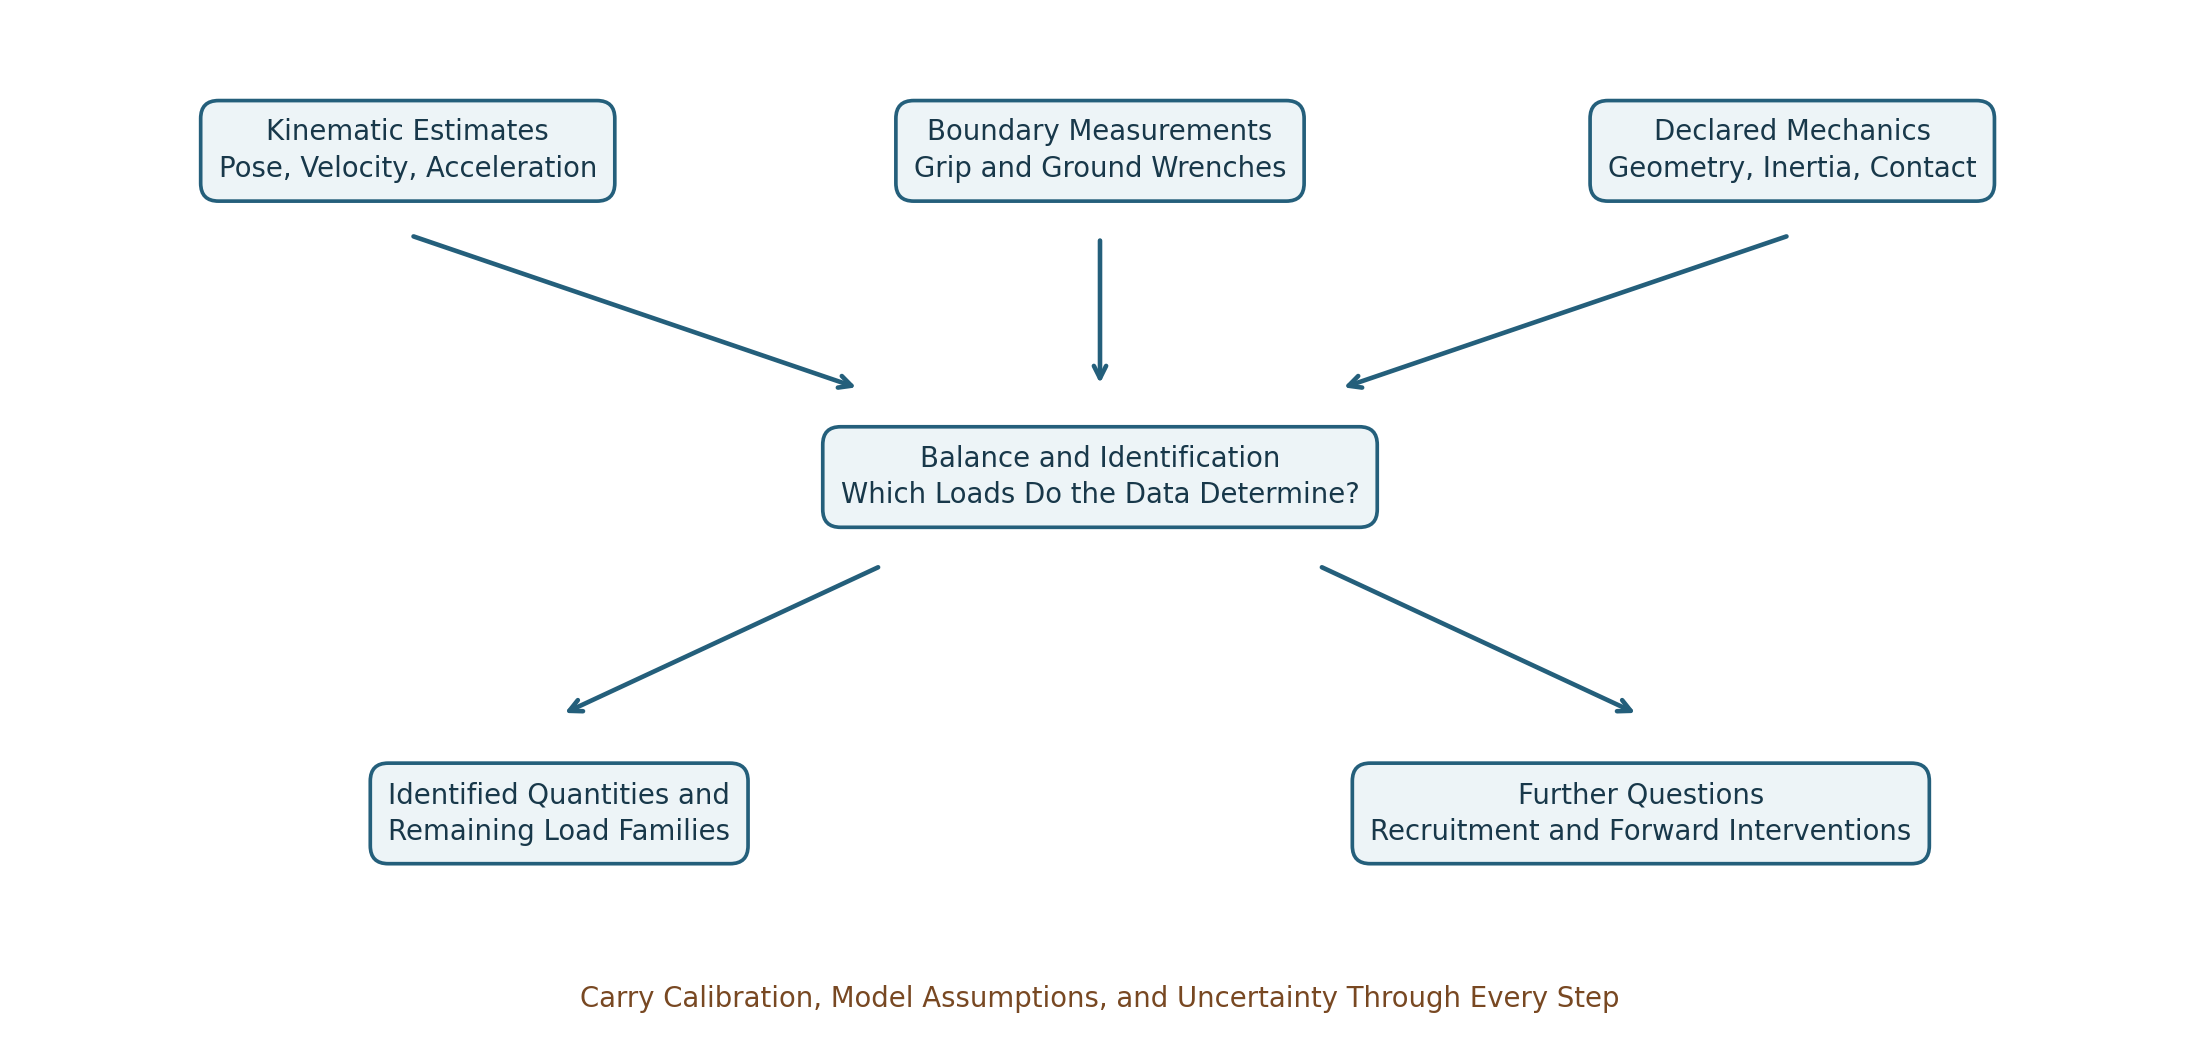
\includegraphics[width=\linewidth]{figures/inverse_identification_workflow.png}
\caption{From Measurements and Declared Mechanics to Identified Loads and Further Research Questions.}
\label{fig:inverse_dynamics_flow}
\end{figure}

\section{Equations, Inputs, and Boundary Conditions}
\label{subsec:canonical_eom}

Use regular local coordinates $q\in\mathbb R^n$ for an articulated-tree model,
with any additional ideal, time-independent closures $\Phi(q)=0$. Let
$J_c=D_q\Phi\in\mathbb R^{k\times n}$ contain independent rows in the contact
mode under consideration. Write
\begin{equation}
 M(q)\ddot q+h(q,\dot q)
 =B(q)u+p(q,\dot q,z)+Q_e+J_c(q)^T\lambda.
 \label{eq:eom_constrained}
\end{equation}
Here $h$ contains the declared inertial bias and gravitational generalized
loads; $u\in\mathbb R^p$ contains the selected applied inputs; $B$ maps them
into generalized loads; $p$ contains separately modeled passive or other
constitutive loads, with internal states $z$ when needed; and $Q_e$ contains
known external loads. A load belongs in exactly one term. Unknown hand or
ground loads cannot be placed in $Q_e$ and simultaneously treated as already
measured. Their parameters must instead join the unknown vector.

For example, a segment wrench maps to generalized load by the transpose of its
compatible velocity Jacobian. Generalized components may have units of force
or moment according to their coordinates; they are not all Cartesian forces.
The matrix often written $C(q,\dot q)$ is a representation of an inertial bias
vector $C\dot q$, not a list of independent physical forces at the hands.

For a regular fully actuated open tree with $B=I$ and known $p,Q_e$, inverse
dynamics evaluates
\begin{equation}
 u=M\ddot q+h-p-Q_e.
 \label{eq:inverse_open}
\end{equation}
There is no mass-matrix inversion in this expression. A positive-definite mass
matrix follows when every nonzero independent coordinate velocity produces
positive kinetic energy in the modeled bodies. Redundant coordinates, massless
idealizations, or a singular coordinate chart require separate treatment. A
straight elbow can make a hand-position Jacobian singular while the physical
joint-space mass matrix remains positive definite.

Even the net load $u$ needs interpretation. A revolute joint's generalized moment
is the load component about its allowed axis; its ideal reaction components
are separate. A full transmitted joint wrench, a generalized joint moment, and
the muscle contribution to that moment are different quantities. Passive tissue
loads already included in the net balance must be subtracted consistently before
calling the remainder active muscle moment.

\section{A Complete Newton--Euler Recursion}
\label{subsec:rnea}

The recursive Newton--Euler algorithm computes open-tree inverse dynamics
without explicitly assembling $M$. Its linear computational cost for a tree
with fixed-size joints does not remove measurement uncertainty or repair an
incorrect contact boundary. The essential ingredients are spatial coordinate
transport, inertial bias, external wrenches, and propagation of child loads.

For one-freedom revolute or prismatic joints, use angular-first spatial motion
$v_i=[\omega_i;v_{O_i}]$ and its power-dual wrench
$w_i=[m_{O_i};F_i]$, both expressed in body frame $i$. Let $\pi(i)$ be the
parent, $X_i$ the motion transform from parent frame to child frame, $S_i$ the
joint motion subspace, and $\mathcal I_i$ the body's spatial inertia about its
frame origin. The fixed-base recursion is
\begin{equation}
 \begin{aligned}
 v_i&=X_i v_{\pi(i)}+S_i\dot q_i,\\
 a_i&=X_i a_{\pi(i)}+S_i\ddot q_i
       +\operatorname{crm}(v_i)S_i\dot q_i,\\
 w_i&=\mathcal I_i a_i+
       \operatorname{crf}(v_i)\mathcal I_i v_i-w_i^{\rm ext}.
 \end{aligned}
 \label{eq:rnea_forward_complete}
\end{equation}
Here $\operatorname{crm}(v)$ is the spatial motion cross-product operator and
$\operatorname{crf}(v)=-\operatorname{crm}(v)^T$ its force counterpart.
For $v=[\omega;v_O]$,
\begin{equation}
 \operatorname{crm}(v)=
 \begin{bmatrix}[\omega]_\times&0\\{}[v_O]_\times&[\omega]_\times\end{bmatrix},
 \qquad [a]_\times b=a\times b.
 \label{eq:spatial_cross_operators}
\end{equation}
Set $v_0=0$ and $a_0=[0;-g]$ to incorporate uniform gravity through this
recursion; do not then subtract gravity again as an external wrench. With this
convention the recursively stored acceleration includes the gravity offset.
For more general joints, include the appropriate joint bias acceleration.
A moving or floating base requires its own specified motion or balance equations.

After forming each body's inertial and external contribution, accumulate from
tips to base:
\begin{equation}
 w_i\leftarrow w_i+\sum_{j:\pi(j)=i}X_j^T w_j,
 \qquad \tau_i=S_i^T w_i.
 \label{eq:rnea_backward_complete}
\end{equation}
The transpose transport follows from power invariance:
$(X_jv_i)^Tw_j=v_i^TX_j^Tw_j$. It carries force-induced moments as well as
rotating components. Adding moments from different points without this transport
loses the lever-arm contribution. These conventions follow the
\href{https://royfeatherstone.org/spatial/v2/}{Featherstone spatial-vector implementation};
its explicit inverse-dynamics recursion also shows the velocity-product terms.

For a closed chain, one may cut a contact to obtain a tree, introduce its unknown
cut wrench, and solve the resulting coupled balance and measurement equations.
A tree algorithm with an arbitrarily assigned cut wrench gives an answer for
that assignment. It does not establish that the assignment was measured or
uniquely implied by motion.

\section{What the Two-Handed Grip Constrains}
\label{sec:loop_closure_formal}

The two hand frames occupy different locations on the club. If $T_C$ is the club
pose and $H_L,H_R$ are fixed hand-to-club attachment transforms under an ideal
rigid grip, closure is
\begin{equation}
 T_L=T_CH_L,\qquad T_R=T_CH_R,
 \qquad T_L^{-1}T_R=H_L^{-1}H_R.
 \label{eq:loop_closure_spatial}
\end{equation}
The final relation supplies six independent local restrictions only where the
chosen representation is regular. Equality of the two hand poses would describe
coincident attachment frames, not the ordinary separated grip. Compliance,
sliding, or changing finger contacts require a different model.

Rigid-body angular velocity is common to its points when expressed in one
frame, but their linear velocities differ:
\begin{equation}
 v_R=v_L+\omega_C\times(r_R-r_L).
 \label{eq:separated_hand_velocities}
\end{equation}
The corresponding acceleration relation includes angular acceleration and
centripetal terms. A Jacobian closure of the form $[J_L,-J_R]\dot q=0$ is valid
only after both Jacobians describe the same transported task frame and point.

The general compatibility equations are
\begin{equation}
 J_c\dot q=0,\qquad
 J_c\ddot q+\dot J_c\dot q=0.
 \label{eq:constraint_acceleration}
\end{equation}
They test whether a candidate trajectory respects the declared constraint;
they contain no independent measurement of $\lambda$.
At constant rank $r$, feasible local configuration dimension is $n-r$.
At a singular point, extra linearized directions need not extend to finite
feasible motions. Low speed at address or transition is not evidence of rank
loss; finite tissue stiffness is not a kinematic rank calculation.

With two seven-coordinate arm models and a regular six-restriction rigid-grip
closure, eight configuration freedoms remain. They include motion of the club.
If the full club-pose task has rank six on the feasible tangent space, only two
posture freedoms remain while holding that task fixed. These counts assume the
specified shoulder bases and arm models; they are not universal counts of the
human body.

Thus $\ker J_c$ contains compatible velocities; task-preserving velocities also
satisfy $J_y\dot q=0$. Neither space says that movement is energetically free.
Grip pressure is a contact-load variable, not a joint velocity. With independent
rows, $\ker J_c^T$ is zero, even though unknown actuator and reaction loads can
still be exchanged without changing the observed motion.

\section{Identification Is a Rank Question}
\label{sec:identifiable}

At a specified state and acceleration, define the known model residual and
unknown vector by
\begin{equation}
 r=M\ddot q+h-p-Q_e,\qquad
 z_\ell=\begin{bmatrix}u\\\lambda\end{bmatrix},\qquad
 A=\begin{bmatrix}B&J_c^T\end{bmatrix},\qquad Az_\ell=r.
 \label{eq:inverse_underdetermined_formal}
\end{equation}
Use $z_\ell$ for load unknowns to distinguish them from constitutive states.
For a consistent linear problem, the solution set is $z_{\ell,0}+\ker A$.
It is a singleton exactly when $A$ has full column rank. Having more unknowns
than equations rules out a unique unconstrained solution; a square matrix alone
does not guarantee uniqueness. Bounds, contact inequalities, and nonlinear
measurements can further restrict the feasible set and must be analyzed as part
of that different problem.

Suppose additional calibrated linear measurements are $Sz_\ell=y_m$. Stack
$A_m=[A;S]$. More sensor channels help identification only when they add
independent information about the unresolved directions. A particular linear
quantity $Cz_\ell$ is identifiable even without the whole vector precisely when
\begin{equation}
 \ker A_m\subseteq\ker C.
 \label{eq:quantity_identification}
\end{equation}
Indeed, all indistinguishable solutions differ by a vector in $\ker A_m$;
the reported quantity is unique only if $C$ annihilates every such difference.
For finite-dimensional linear maps this is equivalent to the rows of $C$ lying
in the row space of $A_m$. Noise replaces an exact affine set by an uncertainty
region; poor singular values then matter as well as rank.

\subsection{An Example Where the Sensor Choice Matters}

Take $M=\operatorname{diag}(2,1)$, $J_c=[1,-1]$, $B=I$, and zero other loads.
For the compatible acceleration $\ddot q=(1/3,1/3)^T$,
\begin{equation}
 \begin{bmatrix}1&0&1\\0&1&-1\end{bmatrix}
 \begin{bmatrix}u_1\\u_2\\\lambda\end{bmatrix}
 =\begin{bmatrix}2/3\\1/3\end{bmatrix}.
 \label{eq:inverse_rank_example}
\end{equation}
Its null direction is $(-1,1,1)^T$. Loads $(1,0,-1/3)$ and $(2,-1,-4/3)$
therefore produce the same acceleration. Measuring $u_1+u_2=1$ adds no rank:
it repeats the sum of the existing equations. Measuring $\lambda=-1/3$ selects
$(u_1,u_2)=(1,0)$ in this ideal example. Measurement precision still limits the
precision of that inference.

If the same mechanism has only one actuator, $B=(1,0)^T$, the inverse matrix
for $(u_1,\lambda)$ is square with determinant $-1$. The corresponding loads
are uniquely determined for this measured acceleration. A loop therefore does
not by itself make inverse dynamics nonunique. Conversely, multiple muscles can
make recruitment nonunique in a completely open limb.

\section{Hand Wrenches and Club Balance}
\label{sec:instrumented_clubs}

A hand's force and moment must be referenced to a point and expressed in a
coordinate frame. Use the same angular-first ordering as the spatial recursion.
For an inertial-frame force $F_i$ and moment $m_i$ about attachment point $i$,
transport to club center of mass $C$ with $r_i=p_i-p_C$:
\begin{equation}
 w_i^C=X_i^*w_i,
 \qquad X_i^*=
 \begin{bmatrix}I&[r_i]_\times\\0&I\end{bmatrix},
 \qquad w_i=\begin{bmatrix}m_i\\F_i\end{bmatrix}.
 \label{eq:hand_wrench_transport}
\end{equation}
Rotate components first if the sensor axes differ from the reporting axes.
The club's net hand wrench is
\begin{equation}
 \begin{bmatrix}
 I_C\alpha+\omega\times(I_C\omega)-m_{\rm other}^C\\
 m_c(a_C-g)-F_{\rm other}
 \end{bmatrix}
 =G\begin{bmatrix}w_L\\w_R\end{bmatrix},
 \qquad G=\begin{bmatrix}X_L^*&X_R^*\end{bmatrix}.
 \label{eq:club_inverse_wrench}
\end{equation}
Here $I_C$ is rotational inertia about the club COM expressed in the same
inertial axes as $\omega,\alpha$; it changes orientation with the club.
The gyroscopic term remains necessary. Other forces include modeled aerodynamic
and impact loads. A moving-grip-point expression $I_{\rm grip}\alpha$ alone
is not a general three-dimensional club balance. During impact, finite sensor
bandwidth and flexible shaft motion may invalidate a simple rigid-body
instantaneous-acceleration estimate; an impulse balance requires its own
interval, boundary, and measurements.

Each $X_i^*$ is invertible, so the full-wrench grasp map has rank six and a
six-dimensional load null space before contact restrictions. Motion can identify
the resultant under the declared model while leaving six combinations of hand
wrenches unresolved. If the model permits only point forces and no hand moments,
the corresponding six-by-six map has rank five at two distinct points. Its one
internal direction is an equal-and-opposite force pair along the line joining
them. A transverse opposing pair produces a couple and is visible in angular
balance. Counting only resultant force misses that distinction.

Arm joint-torque vectors live in their own generalized-coordinate spaces.
For a six-coordinate two-arm model, its six required joint loads cannot be
written as the sum of two three-component hand forces. Hand wrenches enter the
arm equations through their Jacobian transposes and the appropriate
opposite-action signs. Equal and opposite numerical joint-torque entries do
not automatically cancel the club wrench.

\subsection{A Transport and Power Check}

Take $r=(0.2,0,0)$ m, $F=(0,100,0)$ N, and a local hand moment
$m=(0,0,3)$ N m. About $C$, the moment is $(0,0,23)$ N m. If
$v_C=(1,0,0)$ m/s and $\omega=(0,0,2)$ rad/s, the hand-point velocity is
$(1,0.4,0)$ m/s. Power computed either way is
\begin{equation}
 m^T\omega+F^Tv_{\rm hand}
 =(m+r\times F)^T\omega+F^Tv_C=46\ {\rm W}.
 \label{eq:wrench_power_example}
\end{equation}
Using the untransported 3 N m moment together with COM velocity would report
6 W and lose 40 W. The discrepancy is a bookkeeping error, not a new energy
source. At an ideal maintained attachment, the equal-and-opposite wrench acting
on the hand has opposite power when both sides use the same contact twist.
It can transfer energy between golfer and club while canceling in the combined
system's internal power balance.

\subsection{What an Instrumented Grip Actually Measures}

A single six-axis sensor below both hands measures a section wrench. After
accounting for the intervening club/grip inertia and other loads, it can
constrain their aggregate action. It generally cannot resolve twelve independent
hand-wrench components merely because it reports six channels. A second
measurement of the same resultant improves precision but adds no independent
load-sharing rank.

Separate mechanically isolated hand interfaces can supply distinct boundary
wrenches. Multiple shaft sections may also distinguish loads if their placement,
section balances, and calibration make the combined observation map informative.
A pressure array usually measures a subset of contact traction; integrating
normal pressure alone does not recover all tangential forces or free moments.
A contact's net wrench also does not uniquely reconstruct the pressure and shear
distribution across the skin.

The experiment must state exactly which bodies lie on each side of each sensor,
where its wrench is referenced, how its axes are registered to motion capture,
and how sensor mass changes the instrumented club's inertia. Timing offsets
between motion and force signals can create apparent balance violations or
false power peaks. Calibration, cross-talk, saturation, bandwidth, hysteresis,
and repeated-load validation belong in the measurement uncertainty.

\section{Sensor Physics With Defined Units}
\label{subsec:strain_gauges}

A bonded resistance strain gauge measures deformation through
$\Delta R/R=\mathrm{GF}\,\varepsilon$ in its calibrated small-strain range.
It measures local strain first; a structural model and calibration map that
strain to a load. Multiple gauges can separate bending, axial loading, and
torsion only if their geometry and calibration support those components.

For a declared Wheatstone bridge, put $R_1$ above $R_2$ in the left divider
and $R_3$ above $R_4$ in the right divider, with excitation $V_{\rm ex}$
from the common top node to the bottom node. Measure left midpoint minus right:
\begin{equation}
 \frac{V_{\rm out}}{V_{\rm ex}}
 =\frac{R_2}{R_1+R_2}-\frac{R_4}{R_3+R_4}
 =\frac{R_2R_3-R_1R_4}{(R_1+R_2)(R_3+R_4)}.
 \label{eq:wheatstone_output}
\end{equation}
Reversing the measurement leads reverses the sign. If only $R_1=R(1+\delta)$
changes and the others equal $R$, then
\begin{equation}
 \frac{V_{\rm out}}{V_{\rm ex}}=-\frac{\delta}{4+2\delta}
 \simeq-\frac{\mathrm{GF}\,\varepsilon}{4}.
 \label{eq:quarter_bridge_example}
\end{equation}
With GF $=2$, strain $500$ microstrain, and 5 V excitation, the exact output
is approximately $-1.249$ mV. Gauge orientation, active bridge arms, temperature
compensation, lead resistance, and self-heating affect the actual installation.
The bridge conventions and calibration choices should be reported, as emphasized
in the \href{https://www.ni.com/getting-started/set-up-hardware/data-acquisition/i/strain-gages}{NI strain-measurement documentation}.

For a piezoelectric material, a constitutive relation in stress-charge form is
\begin{equation}
 D=d\,\sigma+\epsilon^T E.
 \label{eq:piezoelectric_relation}
\end{equation}
$D$ is electric displacement (charge per area), $\sigma$ is stress, $E$ is
electric field, and $d$ is the piezoelectric coupling tensor under the stated
material convention. This is not an equation for voltage. In a calibrated
one-dimensional approximation, generated charge is $Q_{\rm ch}=d_FF$. An ideal
open-circuit voltage magnitude is $Q_{\rm ch}/C$ for the relevant capacitance; an
ideal inverting charge amplifier gives $V_{\rm out}=-Q_{\rm ch}/C_f$ over its operating
band. For $d_F=4$ pC/N and $F=100$ N, the charge is 400 pC: this corresponds
to 2 V across 200 pF or $-0.4$ V with a 1 nF feedback capacitor. These are
illustrative circuit values, not a specification for a particular instrument.

Leakage, amplifier time constants, and insulation limit sustained measurements;
preload and mounting affect the force path and dynamics. Piezoelectric systems
can measure dynamic and suitably conditioned quasi-static loading. They are
not universally faster or more sensitive than every strain-gauge system.
See the \href{https://www.kistler.com/GB/en/cp/piezoelectric-force-sensors-9224a/P0001619}{Kistler force-sensor documentation}
for the distinction between a sensor's calibrated force response and its
measurement conditions. Six independent load components require an appropriate
mechanical and electrical sensing map, not necessarily six crystals or a hexapod.

\section{Optimization Selects a Hypothesis}
\label{subsec:approach_optimization}

When measurements leave a load family, optimization can select a member. It
adds a criterion; it does not turn the selected member into an observation of
neural intent. State the decision variables, units, constraints, physiological
bounds, and whether the objective is a hypothesis or a computational regularizer.

For example, minimize
\begin{equation}
 \frac12(z_\ell-z_0)^TW(z_\ell-z_0)
 \quad\text{subject to}\quad A_mz_\ell=b_m,
 \qquad W\succ0.
 \label{eq:weighted_load_optimization}
\end{equation}
Here $z_0$ is a declared reference load vector, not a measured fact unless it
actually is measured. For full-row-rank $A_m$, stationarity of the Lagrangian
and substitution into the constraints give
\begin{equation}
 z_\ell^*=z_0+W^{-1}A_m^T
 (A_mW^{-1}A_m^T)^{-1}(b_m-A_mz_0).
 \label{eq:weighted_load_solution}
\end{equation}
Redundant consistent rows can be removed or handled with an appropriate
pseudoinverse. Inconsistent noisy measurements require a residual or statistical
model rather than exact constraints that cannot all hold. Contact bounds and
nonlinear muscle laws alter the optimization problem and may destroy feasibility
or convexity; a numerical optimizer returning a vector is not proof of a valid
physiological solution.

In a deliberately scalar example, $u_L+u_R=10$ N m. Equal weights choose
$(5,5)$ N m. Minimizing $u_L^2+4u_R^2$ chooses $(8,2)$ N m, with objective
80 in the declared squared-moment units. The balance did not change; the
preference did. A proper norm needs scaling when the vector mixes force,
moment, or different capacity scales. Squared joint moment is not metabolic
power. The sum of measured EMG amplitudes is constant with respect to unknown
loads and cannot select a solution unless an explicit decision-dependent
measurement or physiological model connects them.

\section{Muscles, Activation, and EMG}
\label{subsec:approach_emg}

Given a net generalized moment, muscle recruitment is another inverse problem.
If $F_m$ collects musculotendon forces and $R(q)$ their moment-arm map, a
simplified moment balance is
\begin{equation}
 \tau_{\rm net}=R(q)F_m+\tau_{\rm passive,other}.
 \label{eq:muscle_inverse_mapping}
\end{equation}
The sign convention for $R$ follows the chosen coordinate and muscle-length
conventions. A muscle spanning several joints contributes to several entries;
net joint moments do not identify all tensile muscle forces when the map has
unresolved directions. Known external hand wrenches improve the joint-load
estimate without automatically eliminating muscle redundancy.

Surface EMG records a superposition of electrical potentials detected through
electrodes and intervening tissue. Its amplitude depends on motor-unit activity
and recording conditions. It is not a direct recording of motor-cortex commands,
activation as used in a muscle model, or contractile force. The
\href{https://pubmed.ncbi.nlm.nih.gov/25277737/}{Farina, Merletti, and Enoka analysis}
explains why neural interpretation requires care. Electrode placement,
cancellation, cross-talk, normalization, fatigue, and tissue motion all matter.
A larger normalized signal in one arm does not compel a larger resultant hand
wrench from that arm.

A model can link processed EMG to excitation with calibration and uncertainty,
then evolve activation and musculotendon states. For example,
\begin{equation}
 \dot a=\frac{e-a}{\tau(e,a)},\qquad
 F_{\rm CE}=F_{\max}a f_\ell(\ell_f)f_v(\dot\ell_f).
 \label{eq:activation_force_chain}
\end{equation}
This illustrative contractile-element relation must be completed with passive
fiber behavior, pennation, tendon mechanics, and force equilibrium or the chosen
dynamic muscle model. It is not by itself a complete musculotendon force law.
The \href{https://opensimconfluence.atlassian.net/wiki/spaces/OpenSim/pages/53090590/First-Order+Activation+Dynamics}{OpenSim activation-dynamics documentation}
explicitly distinguishes excitation from activation. Different force-length and
force-velocity states can produce different forces at the same activation.

EMG-informed modeling can be quantitatively useful when calibrated and validated;
calling EMG merely qualitative would also be too strong. Report which muscles
are observed, which deep or unmeasured muscles remain free, the activation and
tendon assumptions, and prediction errors on independent conditions. Neither
an EMG ratio nor a minimum-activation objective uniquely establishes how two
hands share a club load without that intervening mechanics.

A model of internal tissue stress requires geometry and constitutive behavior
in addition to boundary loads. An internal-load ambiguity identifies a limit
on inference, not an injury diagnosis or a universal coaching prescription.

\section{Ground Loads and Segment-by-Segment Balance}
\label{sec:lower_body_inverse_dynamics}

Separate calibrated force plates can provide a wrench for each foot when each
foot's contact belongs to its assigned plate and all relevant contacts are
captured. One plate under both feet usually gives their combined wrench; it
does not generally determine the bilateral split. Vertical force alone is less
information than a full force-and-moment measurement.

For a segment with COM $C$, known distal wrench $(F_d,m_d)$ at point $d$, and
unknown proximal wrench $(F_p,m_p)$ at point $p$, all acting on the segment in
inertial axes, the balances are
\begin{equation}
 \begin{aligned}
 F_p&=m(a_C-g)-F_d-F_o,\\
 m_p&=I_C\alpha+\omega\times(I_C\omega)-m_d-m_o^C\\
    &\hspace{1em}-(p_d-p_C)\times F_d-(p_p-p_C)\times F_p.
 \end{aligned}
 \label{eq:distal_proximal_balance}
\end{equation}
$F_o,m_o^C$ collect any other nongravitational external loads with moments
already referenced to $C$. The segment's moment about its COM includes the
moment arms of both distal and proximal forces. To proceed from foot to shank
to thigh, reverse the interaction wrench on the neighboring segment and
transport it to the appropriate point. Passing only an ankle torque upward
while omitting its joint force is incomplete.

These equations estimate a transmitted net wrench under the segment model.
Projecting onto a declared joint axis gives its generalized moment. Anatomical
axis definitions, soft-tissue artifact, joint-center locations, inertial
parameters, and synchronization affect the result. The estimate does not assign
all of that wrench to one muscle or one tissue.

\subsection{Yaw Moment Is Not a Vertical Force Offset}
\label{sec:ground_torque_detailed}

For a force $F$ at COP $r_{\rm COP}$ and a free moment $T_{\rm free}$,
the moment about a reporting point $P$ is
\begin{equation}
 M_P=(r_{\rm COP}-r_P)\times F+T_{\rm free}.
 \label{eq:ground_torque_offset}
\end{equation}
In right-handed axes with $z$ vertical, its yaw component is
\begin{equation}
 (M_P)_z=(x_{\rm COP}-x_P)F_y
 -(y_{\rm COP}-y_P)F_x+(T_{\rm free})_z.
 \label{eq:ground_torque_cop}
\end{equation}
A purely vertical force at a horizontal offset creates roll/pitch moments,
not yaw. For $r=(0.2,-0.1,0)$ m and $F=(0,0,1400)$ N,
$r\times F=(-140,-280,0)$ N m. A reported plate moment about its origin
must be distinguished from the free moment after moving the resultant to COP.
Vendor signs and whether the wrench is force-on-plate or force-on-golfer must
be converted consistently.

For a 100 kg system, 1400 N is about 1.43 body weights using $g=9.81$ m/s$^2$.
If it is the only nongravitational vertical force on that system, its COM
vertical acceleration is $1400/100-9.81=4.19$ m/s$^2$. Neither this force nor
an 80 N m free moment alone determines pelvis acceleration. Dividing 80 N m
by a declared 2 kg m$^2$ fixed-axis inertia gives 40 rad/s$^2$ for that isolated
toy rotation, not a torque and not a complete multisegment pelvis model.

Whole-body angular momentum about the whole-body COM changes with the net
external moment. Pelvis angular momentum also exchanges with legs and trunk
through internal interactions. Different segments can counter-rotate while
preserving whole-body angular momentum. A ground-moment contribution assigned
to a pelvis coordinate therefore depends on the coupled dynamics and the
chosen decomposition; it is not read directly from a force plate.

\subsection{Momentum Exchange and Mechanical Power}

At an ideal stationary no-slip contact on a rigid stationary ground, the contact
velocity is zero, so contact force supplies zero mechanical power there. It
can nevertheless change the golfer's momentum and permit muscle work to be
expressed as segment and club motion. Real shoe deformation, sliding, moving
supports, and contact compliance require their actual velocities and energy
terms. A force multiplied by COM velocity gives a contribution to COM
translational kinetic-energy rate, not automatically the work rate at the
physical contact.

Assigning active ground power to every downswing and passive ground braking
to every follow-through combines unsupported physiological interpretation with
an incorrect contact-power shortcut. Measure the moment direction, state the
system boundary, and compute power with its conjugate velocity. The energy
source, route of transfer, and momentum constraint are related but distinct
parts of the swing explanation.

\section{Conditioning and Measurement Uncertainty}

Inverse dynamics often uses acceleration estimates, so differentiation quality
matters. Independent position-sample errors of variance $\sigma_q^2$ passed
through the centered second difference have acceleration-error variance
$6\sigma_q^2/\Delta t^4$. Real smoothing and correlated errors change this
expression. It illustrates why quoting frame rate alone does not establish
acceleration precision. Filtering choices should be evaluated against relevant
motion and force bandwidth, not chosen solely to make torque traces smooth.

For an open-tree net-load evaluation at fixed model parameters, a first-order
perturbation includes
\begin{equation}
 \delta\tau=M\,\delta\ddot q+(\delta M)\ddot q+
 \delta h-\delta p-\delta Q_e.
 \label{eq:inverse_uncertainty}
\end{equation}
Cross-correlations matter when these quantities come from the same fitted
trajectory. Covariance propagation or repeated sampling through the complete
pipeline is preferable to treating all errors as independent by default.
Model discrepancy and missing external loads are not necessarily random
measurement noise.

\subsection{A Counterexample to the Small-Inertia Argument}

Let $M=\operatorname{diag}(1,\epsilon)$ in consistent coordinate and inertia
units, $0<\epsilon\leq1$. Its two-norm condition number is $1/\epsilon$.
But for a fixed acceleration error $(0.1,0.1)^T$,
\begin{equation}
 \delta\tau=M\,\delta\ddot q=(0.1,0.1\epsilon)^T.
 \label{eq:inverse_error_counterexample}
\end{equation}
The second torque error is 0.01 at $\epsilon=0.1$ and 0.001 at
$\epsilon=0.01$. It decreases. By contrast, a fixed torque error
$(0.1,0.1)^T$ in a forward solve produces acceleration error
$(0.1,0.1/\epsilon)^T$, whose second component increases. The condition number
describes relative worst-case sensitivity with the specified norm and scaling;
it is not the absolute gain of every inverse-dynamics perturbation.
A matrix $1000I$ has condition number one yet multiplies an absolute
acceleration error by 1000 in a load evaluation.

For a planar two-link arm with uniform links, each of unit length and unit mass,
at a straight configuration the joint inertia and endpoint-position Jacobian
can be
\begin{equation}
 M=\begin{bmatrix}8/3&5/6\\5/6&1/3\end{bmatrix},
 \qquad J_y=\begin{bmatrix}0&0\\2&1\end{bmatrix}.
 \label{eq:straight_arm_inertia}
\end{equation}
The task Jacobian has rank one; the mass matrix has positive diagonal entries
and determinant $7/36>0$. The endpoint singularity has not made the joint
inertia singular. In constrained and sensor-augmented inverse problems, inspect
the correctly scaled identification matrix and its singular values as well as
the underlying inertial model. State angle/translation scaling before comparing
condition numbers across models.

\section{Forward Dynamics and a Declared Counterfactual}
\label{sec:ztcf_forward_dynamics}

For specified inputs, constitutive states, and external loads, the acceleration
and ideal reaction in a fixed contact mode satisfy
\begin{equation}
 \begin{bmatrix}M&-J_c^T\\J_c&0\end{bmatrix}
 \begin{bmatrix}\ddot q\\\lambda\end{bmatrix}
 =\begin{bmatrix}Bu+p+Q_e-h\\-\dot J_c\dot q\end{bmatrix}.
 \label{eq:forward_wellposed}
\end{equation}
If $M\succ0$ and $J_c$ has full row rank, the matrix is nonsingular. To see
this, a homogeneous solution obeys $M\delta a-J_c^T\delta\lambda=0$ and
$J_c\delta a=0$. Multiplying the first equation by $\delta a^T$ gives
$\delta a^TM\delta a=0$, so $\delta a=0$ and then $\delta\lambda=0$.

This proves unique instantaneous acceleration for those inputs. Local trajectory
existence and uniqueness also require compatible initial conditions and
sufficient regularity of the reduced differential equations and input policy.
A smooth fixed-mode vector field is locally Lipschitz; contact switching,
friction, impacts, and rank changes require event laws and a fresh analysis.
Matrix invertibility at one instant is not a global guarantee for an entire
swing.

\subsection{Same-State Acceleration and a Forward Branch}

A zero-torque counterfactual (ZTCF) must specify which input is set to zero.
Zero commanded joint torque, zero muscle excitation, zero activation, and
removal of muscle/tissue forces are different interventions. In an effective
joint-input model, setting $u=0$ retains the stated $p,Q_e,h$ laws and their
states. If preload or activation-dependent impedance is not measured, the
baseline inherits that uncertainty. Gravity can be computed from geometry and
mass assumptions; that does not make every elastic or physiological drift term
observable from skeletal motion.

At the same complete state and fixed mode, with other loads held under the
same law, write the acceleration map as
\begin{equation}
 \begin{aligned}
 a(q,\dot q,z,u)&=a(q,\dot q,z,0)+K(q)B(q)u,\\
 K&=M^{-1}-M^{-1}J_c^T(J_cM^{-1}J_c^T)^{-1}J_cM^{-1}.
 \end{aligned}
 \label{eq:same_state_control_effect}
\end{equation}
This identifies the input's acceleration effect under the model. Even if it
is known exactly, $KBu$ need not identify $u$, because projection and actuator
redundancy can remove load directions. Reactions must be recomputed when the
input changes. Retaining measured reactions while zeroing $u$ generally breaks
constraint compatibility.

A forward ZTCF instead starts at the chosen initial state and integrates the
zero-input policy along its own trajectory. It recomputes geometry, inertia,
velocity bias, passive states, reactions, and events along that branch. Once it
has diverged from the actual trajectory, subtracting the two accelerations no
longer compares the same state. Multiplication by one trajectory's $M$ cannot
undo that difference or recover muscle torques.

For an unconstrained dimensionless toy oscillator,
\begin{equation}
 \ddot q=-q+u,\qquad q(0)=\dot q(0)=0,
 \qquad q_{u=1}(t)=1-\cos t,\quad q_{u=0}(t)=0.
 \label{eq:forward_branch_counterexample}
\end{equation}
At $t=\pi/2$, the two trajectories' accelerations are both zero, although the
actual input remains one. The acceleration difference across branches is zero;
the same-state difference is $0-(-1)=1$. This elementary example shows why a
trajectory residual is a model intervention outcome, not an instantaneous
input reconstruction.

For finite-horizon clubface or speed outcomes, compare the outcomes of the two
branches with their uncertainty and initial-state matching explicitly stated.
When using a local variational approximation instead, propagate perturbations
along its evolving baseline and identify its validity range. A forward
counterfactual asks a useful different question from inverse muscle inference;
it is not universally more accurate simply because it runs forward.

\section{A Golf Study That Can Distinguish Explanations}
\label{sec:synthesis_inverse_dynamics}

Suppose the question is whether two movement patterns achieve similar club
outcomes through different hand loading, and whether an effective zero-input
branch predicts different continuation of the motion. A defensible study can
connect these questions without treating any one measurement as sufficient.

\begin{enumerate}
\item Define the primary output: for example, clubhead velocity and face
      orientation just before impact, a net hand-wrench time history, or work
      transferred to the club over a specified interval. Define tolerances for
      calling two outcomes similar and distinguish impact conditions from ball
      flight, which also depends on collision and aerodynamic variables.
\item Specify the body graph, joint coordinates, separated grip frames, club
      flexibility assumptions, contact modes, inertial parameters, and input
      channels. Validate measured trajectory compatibility; report closure
      residuals instead of hiding them inside large artificial reactions.
\item Calibrate and synchronize kinematics, bilateral ground wrenches, and the
      selected grip measurements. Derive the augmented identification map and
      show which quantities are determined. Reserve measured channels or trials
      for validation rather than using all data both to fit and to confirm.
\item Solve the declared net-load problem and test segment and whole-system
      force, moment, and power balances. Propagate plausible measurement and
      parameter variation. If competing load distributions remain possible,
      report that family or interval rather than only one optimizer output.
\item Add muscle modeling and EMG only for the recruitment questions they can
      inform. Compare alternative calibrated recruitment assumptions and
      inspect prediction error on independent data. Do not translate inferred
      muscle forces into tissue stress or injury likelihood without the
      additional validated model required for that output.
\item Branch the forward counterfactual from a declared event or state, specify
      zeroed inputs and retained states, and integrate each branch independently.
      Report the event rules, numerical convergence, and uncertainty in its
      endpoint. Compare models and repeat the analysis across trials before
      drawing a general conclusion about a golfer or a population.
\end{enumerate}

This links geometry to admissible motion, dynamics to required net loading,
measurement to identification, muscle models to recruitment hypotheses, and
power balance to energy transfer. The central scientific gain is an argument
that makes clear what would change its conclusion. A successful fit to one
swing is useful evidence about that fitted model; independent predictions and
controlled comparisons are needed for stronger claims about strategy or benefit.

\section{Chapter Exercises}

\begin{enumerate}
\item Verify the two-coordinate inverse matrix's null vector. Compare ranks
      after measuring the actuator sum, measuring the multiplier, and removing
      the second actuator.
\item Derive wrench transport from invariant power. Reproduce the 46 W example
      and identify the lost lever-arm term when reference points are mixed.
\item Derive grasp-map ranks for two full hand wrenches and for two separated
      point forces. Explain why a transverse opposing force pair creates a couple.
\item Derive the weighted minimum from its Lagrangian and verify $(8,2)$.
      Explain why the selected objective does not establish neural intent.
\item Derive the bridge voltage from its divider voltages and reverse the output
      leads. Convert the piezoelectric charge using each stated capacitance.
\item Reproduce the inverse and forward error calculations for
      $M=\operatorname{diag}(1,\epsilon)$. Verify the straight arm's singular task
      Jacobian and positive-definite inertia.
\item Use the oscillator solution to compare cross-branch and same-state
      acceleration differences at $t=\pi/2$. State what each comparison holds fixed.
\item A paper reports separate left and right spinal muscle moments. Identify
      required boundary loads, moment arms, physiological laws, and independent
      measurements. Explain why muscle redundancy needs no spinal kinematic loop.
\item Design a sensor addition for a remaining golf load-sharing null direction.
      State its rank benefit, calibration needs, and a quantity it cannot identify.
\end{enumerate}
